
\begin{table}[t]
\centering
\caption {Notations}
\scalebox{0.7}{
 \begin{tabular}{l|l}  \toprule
 \multicolumn{1}{c}{\textbf{Symbol} } &  \multicolumn{1}{c}{\textbf{Explanations}}\\\midrule
\textbf{Boldface}& \text{- represents encrypted data}\\
$\tilde{}$ & \text{- represents one-hot-coding}  \\  $\hat{}$ & -represents a differentially private output  \\ $A$ &- an attribute  \\ $s_A$ &- size of domain of attribute $A$
\\$dom(A)=\{v_1,\ldots,v_{s_A}\}$ & - domain of attribute $A$\\ $ct_{A,i}$  &- \# \text{records with value $v_i$ for attribute} A\\ $m$   &-\text{\# number of data onwers}\\ $\boldsymbol{\tilde{\mathcal{D}}}$  &- \text{encrypted database with records in}\\&\text{  per-attribute one-hot-coding } \\ %$\mathcal{A}=\{\mathcal{A}_1,...\mathcal{A}_l\}$   &- \text{set of attributes in the schema of $\boldsymbol{\tilde{\mathcal{D}}}$}\\
$x \times y \text{ table } \mathbf{T}$   &- \text{an encrypted table  with $x$ records in}\\&\text{ one-hot-coding and $y$ columns one for}\\&\text{ each attribute; serves as one of the }\\&\text{ inputs to a transformation primitive}\\ $\mathbf{B}$&- \text{A $m$ - lengthed vector such that each entry}\\&\text{ $\textbf{B}[i]$ represents whether record $r_i, i \in [m]$}\\& \text{is relevant to the program at hand} \\ $V$ & -\text{represents a vector}\\$c$ &- \text{represents a scalar}\\$\mathcal{P}$ & - \text{represents a set}\\
 \bottomrule
 \end{tabular}}
 \label{Notations}
\end{table}

%$Attribute(\phi)$ - The set of attributes that appear in the boolean condition $\phi$\\
%$\mathcal{I}(A)$- Denotes the integral representation of $dom(A)$\\$\mathcal{I}_A(\phi)$- Denotes the elements in $\mathcal{A}$ that satisfies $\phi$


\section{System Overview}

\begin{figure}
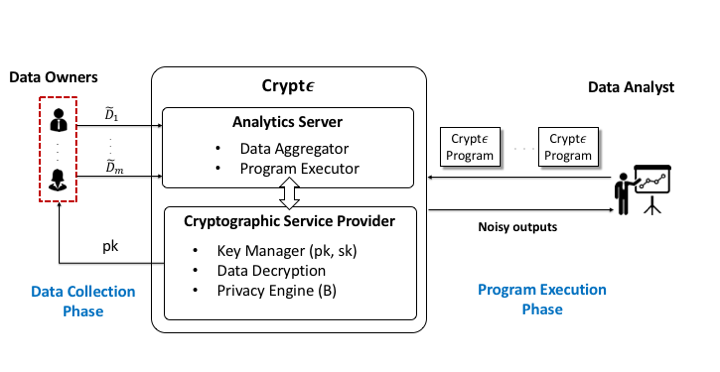
\includegraphics[width=\columnwidth]{cryptE_pic.png}\caption{ Crypt$\epsilon$ System Setting: The  \textsf{AS} runs the Crypt$\epsilon$ programs. The \textsf{CSP} manages the cryptographic primitves. } \end{figure}
This section provides an overview of \system. We begin this section with the desiderata for \system that motivates our design followed by a discourse on the different components of \system and their functionality. Next we discuss about a few additional architectural choices we make for \system. This is followed by a description of \system's trust model and security sketch.
\subsection{Crypt$\epsilon$ Design}
The  desiderata for  the functionality of \system are as follows
\squishlist \item The architecture of \system should be able to support any differentially private algorithm that is permitted in the \textsf{CDP} model at the same order of accuracy guarantee as that of \textsf{CDP}, i.e. constant $O(\frac{1}{\epsilon})$ error bound.
\item Raw data records cannot be stored in the clear in any server, i.e., the server(s) in \system are untrusted. 
\item Data owners must be  off-line.\squishend
Recall from our discussion in section 1, \textsf{CDP} gives constant error bounds, however it relies on a trusted server for this. In contrast \textsf{LDP} requires no trusted server but results in limited accuracy.  The first two principles thus capture \system's objective of achieving the "best of both worlds", i.e., the accuracy guarantees and expressibility of the \textsf{CDP} model with the trust assumptions similar to that of the \textsf{LDP} model. The third principle stems from the fact that another undesirable trait of \textsf{LDP} is its inherent requirement for the data owners to be on-line during every query processing.  It is so because  in \textsf{LDP} %the private data of the individuals are not collated at a single place and hence%
depending on the query at hand, every time the data owners need to compute a different noisy measurement that best answers it. This is in general a poor practice as maintaining active communication channels for the data owners might be unwieldy. \par The first desideratum can be achieved if we collate the data into a single data set such that any measurement can be performed on the entire data set at once followed by a single instance of noise addition as opposed to aggregation over noisy measurements on individual data. The second desideratum mandates that the data hence collected should be suitably protected via cryptographic primitives (e.g. encryption scheme). Thus the first two requirements combined, necessitates \system to be able to perform differentially private computations on the encrypted data itself. This leads us to use linear homomorphic encryption and secure computation (specifically Yao's garbled circuits)  as the cryptographic primitives of our choice for \system. Hence by virtue of secure computation, we can potentially implement all the functionalities of the \textsf{CDP} model in \system. However, bearing the practical efficiency of the cryptographic primitives in mind, we impose certain limitations on the expressibility of \system. Due to the third desideratum, a generic $m+1$ party secure computation is ill-suited for our setting. This requires a third party entity that can factor out the onus of participating in a secure computation protocol from the data owners and capture its functionality in (at least) a 2-party protocol instead.   Moreover, since the data owners are no longer in the loop to monitor every query answering, the aforementioned entity should also watchdog the overall privacy budget expenditure. 
Guided by the above principles we design a two-server model for \system with the following components
\\(1)\textbf{ Data-Owners (\textsf{DO})}-  Each data-owner $\textsf{DO}_i, i \in [m]$ has  a
private data record $D_i$ and is willing to share it only if encrypted.   \\(2)\textbf{ Analytics Server (\textsf{AS})} - The \textsf{AS} wants to run a set of differentially private programs on the dataset $\mathcal{D}=\bigcup_{i=1}^m D_i$  but has 
access only to the encrypted copies of $D_i, i \in [m]$.
\\(3)\textbf{ Cryptographic Service Provider (\textsf{CSP})} -
 The \textsf{CSP} manages the cryptographic primitives used in Crypt$\epsilon$ and interacts with the \textsf{AS} to compute the
noisy answers. It is also responsible for monitoring the privacy overall budget expenditure.
%\xh{Rather than providing all the encryption details, can we just simply have an algorithm box to summarize the interactions between these three components. Then describe the interactions and highlight the key functionalities of each component, and then the trust model. }

 
 
\subsection{Crypt$\epsilon$ Modules}

\stitle{Cryptographic Service Provider (\textsf{CSP})}\\
(1)\textbf{ Key Manager }- The foremost duty of the \textsf{CSP} is to initialize the encryption scheme of Crypt$\epsilon$. This task is handled by the \textit{Key Manager} module which generates the key pair $(sk,pk)$ for the \textsf{labHE} scheme. It stores the secret key, $sk$ with itself and releases the public key, $pk$. Note that since only the \textsf{CSP} has access to the secret key $sk$, it is the only entity capable of decryption in Crypt$\epsilon$.\\
(2)\textbf{ Data Decryption }- The \textsf{CSP} being the only entity capable of decryption,  any measurement of the data (even noisy) has to involve the \textsf{CSP}. The \textit{Data Decryption} module is tasked with handling all such interactions with the \textsf{AS}. \\
(3)\textbf{ Privacy Engine }- Crypt$\epsilon$ starts of with a total privacy budget of $\epsilon^B$ which is unanimously agreed upon by all the data owners. Note that the mechanism of deciding $\epsilon^*$ should be piloted by social prerogatives \cite{e1,e2} 
and is currently outside the scope of Crypt$\epsilon$. For executing any program, the \textsf{AS} has to interact with the \textsf{CSP} at least once (for decrypting the noisy answer) thereby giving the \textsf{CSP} the opportunity to monitor the \textsf{AS}'s actions in terms of privacy budget expenditure. The \textit{Privacy Engine} module hence maintains a public ledger that records the privacy budget spent in executing each individual program. Once the privacy cost incurred reaches 
$\epsilon^B$, the \textsf{CSP} refuses to decrypt any further answers thereby ensuring that the privacy budget is not exceeded.  The ledger is completely public allowing any data owner to verify it as and when desired.\\
\stitle{Data Owners (\textsf{DO})}\\
(1)\textbf{ Data Encoder} -  Each data owner $\textsf{DO}_i, i \in [m]$ has a private data record $D_i$ of the form $\langle A_1,...A_l\rangle$ where ${A}_j$ is an attribute. At the very outset, every data owner  $\textsf{DO}_i$ represents his/her private record $D_i$ in its respective per attribute one-hot-coding format. The one-hot-coding is a way of representation for categorical attributes and is illustrated by the following example. 
If the database schema in \system is given by  $\langle Age,Gender\rangle$ then corresponding one-hot-coding representation for a data owner $DO_i, i \in [m]$ with the record $\langle 30, Male\rangle$, is given by $\tilde{D_i}=\langle[\underbrace{0,\ldots,0}_{29},1,\underbrace{0,\ldots,0}_{70}],[1,0]\rangle$. \\
(2)\textbf{ Data Encryption} - The \textit{Data Encryption} module stores the public key $pk$ of the labHE scheme used in Crypt$\epsilon$ which is announced by the CSP. This key is used for an element-wise encryption of the data owners encoded record of per attribute one-hot-codings. In our aforementioned example, we get $\mathbf{\tilde{D}}=\langle[\underbrace{labEnc_{pk}(0),\ldots}_{29},labEnc_{pk}(1),\\\underbrace{\ldots,labEnc_{pk}(0)}_{70}],
[labEnc_{pk}(1),labEnc_{pk}(0)]\rangle$. Finally the data owner sends this encrypted record to the \textsf{AS} via a secure channel.This is the only interaction that a data owner ever participates in, all the program executions are carried out by the \textsf{AS} and the \textsf{CSP} with the data owners being completely off line.\\
\stitle{Analytics Server (\textsf{AS)}}\\
(1)\textbf{  Aggregator} - The \textit{Aggregator} collects the encrypted records $\mathbf{\tilde{D_i}}$ from each of the data owners $\textsf{DO}_i$ and collates them into a single encrypted database $\boldsymbol{\tilde{\mathcal{D}}}$. %Note that in contrast, the server in the \textsf{CDP} model, being trusted, stores the data in the clear whereas in the \textsf{LDP} model the untrusted server stores appropriately randomized (noisy) data.   
\\(2)\textbf{ Program Executor }- The \textit{Program Executor} is the most important module of the \textsf{AS} and is tasked with the execution of Crypt$\epsilon$ programs. It takes as input a Crypt$\epsilon$ program from an external analyst, alongside the appropriate privacy parameter $\epsilon$ and publishes the differentially private output computed with the assistance of the \textsf{CSP}. Crypt$\epsilon$ supports a set of 9 primitives and a Crypt$\epsilon$ program is an execution plan expressed as a sequence of these primitives. The primitives can be broadly classified into two types- transformation primitives and measurement primitives. Transformation primitives allow certain modifications on the encrypted data and are performed almost entirely by the \textsf{AS}. The measurement primitives on the other hand reveal some noisy measurement of the data and requires interaction with the \textsf{CSP}. \system supports two types of measurement primitives that implement two of the most popular differentially private mechanisms, Laplace mechanism \cite{Dork} and NoisyMax \cite{Dork}. A typical Crypt$\epsilon$ program execution consists of  a series of transformation on the encrypted data followed by a measurement primitive and arbitrary post-processing. \\
\textit{Noise Addition in \system} - For the Laplace mechanism, both the \textsf{AS} and the \textsf{CSP} add two separate instances of the random noise to the program output. This is necessary because had only one of them added the noise, then after the release of the clear text output, that party can simply subtract out the noise to reveal the true private answer. An alternative way can be both \AS and \CSP jointly computing a single instance of the noise using a secure computation protocol (see Appendix D.1). However, we do not implement it in the current version of \system as the two-fold noise addition is more efficient. For the NoisyMax primitive, we provide an efficient secure computation protocol where only a single instance of noise by either party suffices. 
Since in Crypt$\epsilon$ the point of noise addition is just at the two servers, unlike at every individual in \textsf{LDP}, we achieve constant error bounds which is of the same order as that of \textsf{CDP} (see section \ref{exp:results}). 
\subsection{Crypt$\epsilon$ Workflow}
The complete workflow of Crypt$\epsilon$ is outlined as follows\\(1) \textbf{ Setup Phase} - This is the very first step in Crypt$\epsilon$ where the key manager of \textsf{CSP} generates the key pair for labHE $(sk,pk)$, publishes $pk$ and stores $sk$. \\(2) \textbf{ Data Collection Phase }- In the next phase, the $\textit{Data 
Encoder}$ and $\textit{Data Encryption}$ modules of every data owner, work to produce the encrypted data records which are then submitted to the \textsf{AS}. The data owners are relieved of all other duties and can go completely off-line. The $\textit{Aggregator}$ module of the \textsf{AS} then aggregates these encrypted records into a single encrypted database $\boldsymbol{\tilde{\mathcal{D}}}$. \\(3) \textbf{ Program Execution Phase} - In this phase, the \textsf{AS} executes a Crypt$\epsilon$ program with some interaction with the \textsf{CSP}  and generates a differentially private output.  \\
The \emph{Setup} and \emph{Data Collection} phases occur just once at the very beginning, every subsequent program  is handled via the corresponding  \emph{Program Execution} phase. Figure 1 shows the diagrammatic representation of \system. A comparative analysis of \system, \textsf{CDP} and \textsf{LDP} is presented in  Table \ref{DPCompare}.
\begin{table}[h!]
\centering
\caption {Comparative analysis of the different DP models}
\scalebox{0.6}{ \begin{tabular}{|l| c c c|}  \toprule
\multicolumn{1}{|c}{\textbf{Features}} & \textbf{LDP}  & \textbf{CDP}  & \textbf{Crypt$\epsilon$}  \\ [0.5ex] 
 \hline \hline\# Servers & 1& 1 & 2\\\hline
Trust  & & & Untrusted \\  Assumption & Untrusted & Trusted & Semi Honest \\for Server &  &   &  Non-Colluding  \\ \hline
Data Storage & \multirow{2}{*}{Noisy} & \multirow{2}{*}{Clear} & \multirow{2}{*}{Encrypted} \\in Server & &  &  \\\hline
Adversary & Unbounded & Unbounded & Bounded \\\hline
 Error & $O\Big(\frac{\sqrt(n)}{\epsilon}\Big)$& $O\Big(\frac{1}{\epsilon}\Big)$ & $O\Big(\frac{1}{\epsilon}\Big)$\\\hline
 Impossibility & Everything & Algorithms w/ & Same as that \\results & beyond SQ model & Unbounded Sensitivity & of \textsf{CDP} in theory \footnotemark\\
  [1ex] 
 \bottomrule
 \end{tabular}}\label{DPCompare}
\end{table}
\footnotetext{For practical constraints the current implementation has restrictions}
 %in between that of the central differential privacy model and the local differential privacy model - although it is definitely much weaker than that of the central differential privacy model, Crypt$\epsilon$'s trust model is slightly stronger as compared to that of the local differential privacy model owing to the aforementioned premises. 
%The formal security analysis for \system is presented in Appendix section B. 
\begin{comment}
learn any other information about the private datasets Di beyond what is revealed by the
model itself. Even in the case that one of the two servers (MLE or CSP) colludes with some
of the data-owners, they should learn no extra information about the data held by the
honest data-owners. In order to achieve this goal we design a system that can be seen as
multi-party protocol run by the m +2 parties mentioned before and specified by a sequence
of steps. This system (described in Section 4) has the following two-phase architecture:
We assume that the Evaluator and the CSP do not
collude. Each one may try to subvert the system as
discussed above, but they do so independently. More
precisely, at most one of these two parties is malicious:
this is an inherent requirement without which security
cannot be achieved.
• We assume that the setup works correctly, that is all
users obtain the correct public key from the CSP. This
can be enforced in practice with appropriate use of
Certificate Authorities.
Note that is true for any cryptographic primitive and is 
The can actually be avoided by removing the . m+1 secure computation where However this is Thus by capturing the we are having an huge efficincy gain now that teh problem is reduced to antwo-party

\subsection{Protocols} \xh{This might go first with the algorithm box or figure.}
In this section, for each of the three entities we list down the interactions that are initiated by them.
\begin{itemize}\item CSP- The foremost duty of the CSP is to initialize the encryption scheme of Crypt$\epsilon$. Specifically the CSP generates the key pair $(sk,pk)$ for the labeled homomorphic encryption. It stores $sk$ with itself and makes $pk$ public. Note that since only the CSP has access to the secret key $sk$, it is the only entity capable of decryption in Crypt$\epsilon$.
\item Data owners- Recall that each data owner owns a single private record which he/she shares with the AS in the encrypted form as follows. First every data owner represents his/her record in its respective per attribute one-hot-encoding format. For example, if the database schema is given by  $D=<Age,Gender>$ then a data owner with the record $<30, Male>$ would firstly represent it as $\mathcal{E}(D)=<[\underbrace{0,\ldots,0}_{29},1,\underbrace{0,\ldots,0}_{70}],[1,0]>$. This is followed by an element-wise encryption of this record of per attribute one-hot-encodings using the pubic key $pk$. In our aforementioned example, we get $\mathbf{D}=<[\underbrace{Enc(0),\ldots}_{29},Enc(1),\underbrace{\ldots,Enc(0)}_{70}],[Enc(1),Enc(0)]>$. Finally the data owner sends this encrypted record to the AS. Note that this is the only interaction that a data owner ever participates in. All the  query answering are carried out by the AS and the CSP with the data owners being completely off line. \item AS - After receiving the encrypted records from each of the data owners, the AS first collates them into a single encrypted database $\mathbf{\tilde{D}}$. For any subsequent query answering, $\mathbf{\tilde{D}}$ is subjected it to a series of transformations most of which are carried out by the AS by itself. However since the CSP is the only entity capable of decryption, for getting any measurement (even noisy) in the clear the AS has to interact with it. There are precisely two types of interactions between the AS and the CSP \begin{enumerate}\item Yao's Garbled Circuit \item Decryption of encrypted noisy value\end{enumerate}\end{itemize}
\end{comment}


\eat{Yet another alternative implementation could have been to engage the $m$ data owners and the \textsf{AS} in a $m+1$ secure computation protocol. This approach has two disadvantages. Firstly, as the number of data owners grow, the communication and computation overheads of this $m+1$ secure computation protocol would get prohibitively high. Secondly, this violates our requirement of off-line data owners. Thus by introducing a separate entity in the form of the \textsf{CSP}, we factor out the onus of participating in a secure multi party computation from the data owners and capture their computation power in a secure protocol between just the \textsf{CSP} and the \textsf{AS} instead %. Note that with the \textsf{CSP} in the picture, the secure computation is now reduced to a two-party case
irrespective of the number of data owners. %Not only does this improve the efficiency of our protocols drastically but is also advantageous from the perspective of ease of system implementation and maintenance. It is so because otherwise we would have had to maintain secure channels between all pairs of data owners, which would become extremely cumbersome with large values of $m$. Moreover all the data owners would have to be online for every program execution. Hence the choice of having a separate server in the form of the \textsf{CSP} is made from the efficiency point of view.
%The second assumption of an computationally bounded adversary is inherent in semantically secure cryptographic protocols. %Another design choice for Crypt$\epsilon$ could have been to keep the data owners in the loop for every program execution such that some of the data transformations could be pushed down to them. Since the data owners can perform the transformations on the plain text and in parallel, this could potentially improve performance. However this would require the data owners to be on-line during the program execution which might be unwieldy in practice especially with a large number of geographically dispersed data owners. 
\par %Keeping the efficiency of our implementation in mind, we used only two instances of simple two-party Yao's garbled circuits for Crypt$\epsilon$. In addition, we propose two optimizations that leverage on the fact that the \textsf{AS} is satisfied with differentially private outputs; this allows  us to expend some of the privacy budget in differentially private pre-processing of the encrypted data. 
The class of programs supported by Crypt$\epsilon$ is any program that can be expressed as a composition of  Crypt$\epsilon$ primitives followed by arbitrary post-processing. Crypt$\epsilon$ supports 7 transformation primitives and 2 measurement primitives. The noisy measurements allowed are the Laplace mechanism and the Noisy max (see section 4.2), two of the most popular and standard differentially private algorithms. The main constraint behind the design of the transformation primitives is that their composition should allow seamless sensitivity analysis.  Sensitivity analysis of arbitrary relational algebraic queries is a hard problem, for e.g. sensitivity of conjunctive counting queries with join operator is unbounded \cite{sensitivity}. Hence all the transformations that Crypt$\epsilon$ supports have bounded stability \cite{PINQ} such that the sensitivity analysis of any program written using them is straightforward. In fact, we showcase that the proposed Crypt$\epsilon$ primitives are indeed very powerful, enabling us to answer practically useful queries, such as linear counting queries etc. 
\\ 
}





\subsection{Trust Model}
Both the servers, \textsf{AS} and \textsf{CSP} are completely untrusted in Crypt$\epsilon$. 
Thus from the data owners perspective the trust assumption is similar to that of \textsf{LDP}; the data owners need not place their trust in any external entity. 
However there are two modest differences in the Crypt$\epsilon$ setting from that of \textsf{LDP}.\\
 (1) We assume that the \textsf{AS} and the \textsf{CSP} are non-colluding and follow the honest-but-curious (or semi-honest) adversary model. %That is, they always follow the instructions of the protocol faithfully but strive to learn extra information about the private records from the messages received during the execution of the protocol. 
 Moreover we assume that each data owner has a private channel with the \textsf{AS}. This is to prevent any third party (including the \textsf{CSP}) from eavesdropping. \\
 (2) The adversary is now reduced to a computationally bounded one as opposed to the information theoretic one  in \textsf{LDP}.
 
 
 \subsection{\system Security Sketch}
 Let $\Pi$ represent the protocol for the end-to-end execution of a $\epsilon$-DP program in \system.  In this paper we consider a
semi-honest adversary  $Adv$ (see section 3.4) who can corrupt any subset of the data owners and at most one of the two
servers. This captures our assumption that the two servers are non-colluding. Thus the requisite security definition should state that $Adv$ only learns the data of the corrupted data owners and the  differentially private output but nothing else about the honest data owners. In other words, the view of the adversary $Adv$ should be computationally indistinguishable from a truly differentially private protocol. 
Let $P$ be a program that is submitted by the data analyst to the protocol $\Pi$ and it is to be run on the data set $\mathcal{D}$ with privacy parameter $\epsilon$. Thus based on our discussion on noise addition in sec 3.2, we define the ideal functionality $\mathcal{F}=(\mathcal{F}_1,\mathcal{F}_2)$ of the protocol $\Pi$ as follows.
\\If $P$ uses Laplace mechanism \cite{Dork}, then
\begin{gather} 
\mathcal{F}_1(P,\mathcal{D},\epsilon)=P(\mathcal{D})+\eta_2\\\mathcal{F}_2(P,\mathcal{D},\epsilon)=P(\mathcal{D})+\eta_1 \\ \eta_1, \eta_2 \sim Lap(\frac{\Delta}{\epsilon})\end{gather}  where  $\Delta$  is the suitable sensitivity of the program. In this case, $output^{\Pi}(\mathcal{D},P)$ which denotes the output of \system that can be published and is given by $P(\mathcal{D})+\eta_1+\eta_2$.\\
If $P$ uses NoisyMax mechanism \cite{Dork}, then
\begin{multline}
\mathcal{F}_1(P,\mathcal{D},\epsilon)=\mathcal{F}_2(P,\mathcal{D},\epsilon)=NoisyMax(P(\mathcal{D}),\Delta,\epsilon) 
\end{multline} where $P(\mathcal{D})$ produces a vector and  $\Delta$ is the suitable sensitivity of the program. $output^{\Pi}(\mathcal{D},P)$ in this case is equal to $NoisyMax(P(\mathcal{D}),\Delta,\epsilon)$.\\
Formally, using the standard simulation based definition \cite{Oded},
\begin{theorem}  Let $S \subset \{1,...,m\}$ then $\Pi$, (i.e. the protocol for an end-to-end program execution in \system) realizes $\mathcal{F}$ (eq 2-6)  with correctness and privacy against
the adversaries $Adv_1=\textsf{AS} \cup \{\textsf{DO}_i, i \in S\} \cup \mbox{Data Analyst}$  and $Adv_2=\textsf{CSP} \cup  \{ \textsf{DO}_i, i \in S\} \cup \mbox{Data Analyst}$
 if there exists  P.P.T algorithms $Sim_1$ and $Sim_2$ such that \begin{gather*} \big\{Sim_1({D_i, i \in S},\mathcal{F}_1(P,\mathcal{D},\epsilon)),\mathcal{F}(P,\mathcal{D},\epsilon)\big\} \\\stackrel{C}{\equiv} \big\{view^{\Pi}_{Adv1}(P,\mathcal{D}),output^{\Pi}(P,\mathcal{D})\big\}  \numberthis\label{adv1}
\\ \big\{Sim_2({D_i, i \in S},\mathcal{F}_2(P,\mathcal{D},\epsilon)),\mathcal{F}(P,\mathcal{D},\epsilon))\big\} \\\stackrel{C}{\equiv}\big\{ view^{\Pi}_{Adv2}(P,\mathcal{D}),output^{\Pi}(P,\mathcal{D})\big\}  \numberthis\label{adv2}
\end{gather*} for all possible inputs  where $ \stackrel{C}{\equiv}$ denotes computational indistinguishability and $view^{\Pi}_i$ denotes the view of entity $i$ in protocol $\Pi$. 
\end{theorem}
\begin{corollary} Protocol $\Pi$ satisfies \textsf{SIM-CDP} \cite{CDP} privacy.\end{corollary}
The proof of this is presented in Appendix A. \eat{Here we just present an intuitive understanding of it. The interactions between the \textsf{AS} and the \textsf{CSP} can be categorised as \\(1) \textsf{CSP} generates garbled circuits with noisy outputs that are evaluated by the \textsf{AS}\\(2) \textsf{AS} sends encrypted masked data to the \textsf{CSP} and gets a transformed encrypted data in response \\(3)\textsf{AS} sends encrypted noisy data and gets back the data in the cleat with additional noise from the \textsf{CSP}\\
The garbled circuits are inherently semantically secure. For the second type of interaction, the random
mask hides the true plaintext
from the \textsf{CSP} while the \textsf{AS} cannot decrypt anything as it does not have access to the secret key $sk$. The last type of interaction outputs a noisy measurement over the data and illustrates the fact that both  \textsf{AS} and \textsf{CSP} add noise to the final answer in \system to ensure that both the servers are allowed only a differentially private  view of the data. Moreover, in
addition to the \emph{Program Executor} module of the \textsf{AS}, the data analyst
communicates the \system program and the privacy parameter $\epsilon$
to the \textit{Privacy Engine} module of the \textsf{CSP}. This enables the \textsf{CSP} to
compute the sensitivity of the program for itself (required while
adding its own noise) thereby thwarting any privacy budget over
expenditure attempts.}
 




\subsection{Discussion on Crypt$\epsilon$ architecture}\label{architecture}
 Crypt$\epsilon$  is based on the premise that there are $m$  data owners, each possessing a private data record, and the \textsf{AS} is the primary entity who is interested in learning certain differentially private statistics on the collective data.  Thus in \system, we require the \textsf{AS} to  shoulder the major chunk of the workload for any Crypt$\epsilon$ program execution; interactions with the \textsf{CSP} should be minimal and only related to data decryption.
Keeping this in  mind, we design the \textsf{AS} to perform most of the data transformations by itself (Table \ref{perf}). Specifically for every Crypt$\epsilon$ program, the \textsf{AS} processes the whole database and transforms it into concise representations (like an encrypted scalar or a short vector) which is then decrypted with the help of the \textsf{CSP}. It is interesting to note that we could have had an alternative implementation for Crypt$\epsilon$ where the private database is equally shared between the two servers and they engage in a secret share based secure computation protocol for computing the differentially private answers. However, this would require both the servers to do almost equal amount of work for every program. Such an arrangement would be justified only if both the servers are equally invested in learning the differentially private statistics and is ill-suited for Crypt$\epsilon$. Additionally, a secret-share based computation would be much more communication intensive resulting in a performance hit. 

The primitives for \system have been designed bearing two things in mind. Firstly, their composition should allow easy sensitivity analysis (for e.g. transformations must have bounded stability). Secondly, all the primitives should have very efficient implementations. Thus although the architecture of \system imposes no fundamental restriction on its expressibility and in theory we can enjoy the same algorithmic power as that of \textsf{CDP}, we restrict the expressibility in the current implementation of \system to ensure practicality of \system programs. Nevertheless, there is a separation between \system and \textsf{LDP} as explained in Appendix D2.


\eat{\begin{table}[h!]
\small
\centering
\caption {Comparative analysis of the different DP models}
 \begin{tabular}{l| c c c}  \toprule
\multicolumn{1}{c}{\textbf{Features}} & \textbf{LDP}  & \textbf{CDP}  & \textbf{Crypt$\epsilon$}  \\ [0.5ex] 
 \midrule \midrule \# Servers & 1& 1 & 2\\\hline
Trust  & & & Untrusted \\  Assumption & Untrusted & Trusted & Semi Honest \\for Server &  &   &  Non-Colluding  \\ \hline
Data Storage & \multirow{2}{*}{Noisy} & \multirow{2}{*}{Clear} & \multirow{2}{*}{Encrypted} \\in Server & &  &  \\\hline
Adversary & Unbounded & Unbounded & Bounded \\\hline
 Error & $O\Big(\frac{\sqrt(n)}{\epsilon}\Big)$& $O\Big(\frac{1}{\epsilon}\Big)$ & $O\Big(\frac{1}{\epsilon}\Big)$\\\hline
 Impossibility & Everything && \\results & beyond SQ model & None & None\footnotemark\\
  [1ex] 
 \bottomrule
 \end{tabular}
\end{table}
\footnotetext{Theoretically no restriction, however practical constraints maybe present}}

%\arc{ Can add another column for Mixnets maybe?}
